\section{Evaluation}
\label{sec:eval}

We evaluate \sys{} on 7 \coq{} specifications of distributed key-value-store consistency: Chapar's published causal-consistency spec~\cite{chapar} and 6 new \emph{\sys{} suite} specs co-developed with a formal-verification and distributed-systems expert (\cref{app:suite}). We extract synthesized implementations from Gallina to OCaml and benchmark them on a 5-VM Google Cloud cluster under a distributed runtime against hand-written expert references. For synthesis, we compare against SOTA coding agents, Codex (GPT-5.4)~\cite{codex} and Claude Code (Opus 4.6)~\cite{claude-code}, under the same prompt and budget. We answer three questions in the following subsections:
\begin{itemize}[leftmargin=*,nosep,itemsep=2pt,topsep=2pt]
\item \textbf{Q1. Does \sys{} handle hard specifications?} \sys{} succeeds on all $7$ in about $6.8$ hours and \$$106$ per spec on average (max $11$h, \$$155$), versus $2$ of $7$ each for Codex and Claude Code under the same prompt and budget (\cref{sec:eval-synthesis}).
\item \textbf{Q2. Are the synthesized implementations performant?} They match or beat every expert-implemented reference: $3\times$ throughput on Chapar's vector-clock reference, $1.4\times$ on \sys{} suite CC and monotonic reads, comparable on read-your-writes (within $20\%$), and sustained throughput on MW and RYW+MW where the reference times out (\cref{sec:eval-perf}).
\item \textbf{Q3. Which of \sys{}' design decisions drive these results?} The joint code-and-proof co-design, the ISA's proposer and reloader roles, the audit step, the \coq{} feedback to the DSA, and the performance feedback to the ISA each contribute consequentially. The DSA alone also sets a new state-of-the-art on four public proof benchmarks across four languages (\cref{sec:eval-ablations}).
\end{itemize}

\subsection{Experimental Setup}
\label{sec:eval-setup}

\textbf{Specifications. \ }
Each specification is a high-level reference implementation of a key-value store; its state type and operations define the consistency notion. \sys{} takes a specification and produces a refining implementation paired with a machine-checked proof of correctness on every input.

Chapar~\cite{chapar} provides a published causal-consistency specification (CC). The other six form the \emph{\sys{} suite} benchmark dataset that we release alongside the system (\cref{app:suite}): read-your-writes (RYW), monotonic writes (MW), monotonic reads (MR), their composition (RYW+MW), and two causal-consistency variants: \sys{} suite CC and LCC (\emph{labeled} causal consistency, where each client subscribes to a set of topic labels and sees causality enforced only on those labels). The \sys{} suite spans the space of session consistency guarantees. To the best of our knowledge, no prior benchmark provides verified \coq{} artifacts across this range.
% 
Difficulty grows in three tiers: simple (RYW, MW), specs whose proofs need many cases (MR, RYW+MW), and specs that also manage explicit dependency sets (CC, LCC).
% through specifications whose proof needs multi-case splits , to specifications that require bridging the implementation's vector clocks to the spec's explicit dependency sets (CC, LCC). 
A side-by-side summary of all seven specifications appears in \cref{app:consistency-specs}.

\textbf{Harness and metrics. \ }
Verified \coq{} implementations are extracted to OCaml (via \coq{}'s built-in extraction, an automatic compilation pass from Gallina to OCaml) and run under a distributed runtime on a 5-VM Google Cloud cluster. Each run executes $4$ parallel workers $\times$ $1{,}000$ random operations; we sweep across put rates, and run a separate scaling sweep at put rate~$=50\%$ over $N \in \{1{,}000, 2{,}000, 5{,}000, 20{,}000\}$. \cref{app:perf-harness} covers the cluster topology and toolchain.
% 
% \mohsen{We already said these in section 3. Commented.}
% A run \emph{closes} a benchmark when \coq{} accepts the proof with no \texttt{Admitted}, \texttt{Axiom}, \texttt{Hypothesis}, or \texttt{Parameter} terms, the audit step (\cref{sec:design-heartbeat}) accepts the candidate, and the extracted OCaml runs on the harness. 
Every method runs under the same per-spec wall-clock and dollar budget. Runs that exhaust either budget are considered failed runs. 
% before closing 
Each cell aggregates three independent runs, and we report pass rate 
% (closures out of three), 
(successes out of three), 
time-to-finish, dollar cost, throughput, p99 latency, peak memory, and ops-per-worker scaling, all as medians.

\textbf{Baselines. \ }
The synthesis baselines are Codex (GPT-5.4)~\cite{codex} and Claude Code (Opus 4.6)~\cite{claude-code}. Both run under the same prompt and budget as \sys{}' DSA, so the comparison isolates the agentic architecture. Codex is also \sys{}' primary backend. 
For performance comparisons, the references are the hand-written expert implementations: 
Chapar's two published references (vector-clock and list-based)~\cite{chapar}, and the expert-written reference released alongside each \sys{} suite specification, except LCC, a custom spec with no expert reference.
% 
For the cross-language evaluation, 
we adopt four public verification benchmarks (DafnyBench, Verus-Bench, miniCodeProps, CoqStoq) across the languages Dafny, Verus, Lean, and \coq{}. 
We compare against the strongest published prior tool for each benchmark.
\cref{app:benchmarks} covers three more (VERINA, AlgoVeri, CloverBench). These cross-language benchmarks target function- and algorithm-level tasks, smaller and simpler in scope than the real-world distributed systems above.

\definecolor{rowhl}{HTML}{EFF3F8}
\definecolor{passgood}{HTML}{C8E6C9}    % darker green for 3/3
\definecolor{passok}{HTML}{E6F4E6}      % light green for 2/3
\definecolor{passfail}{HTML}{F8D7DA}    % light red for <2/3
\definecolor{rulecol}{HTML}{B0B7BF}     % light gray for vertical rules

% [addressed in caption] \ak{You're missing a crisp statement somewhere on the takeaway from this big table. We need it somewhere, don't leave it to the reader to try to parse out. "Overall, \sys succeeds at a much higher rate, succeedign near every time, at a lower cost, in fewer hours than previous attainable. This holds across \textit{all} specifications we tried.}}
\begin{table}[t]
\centering
\footnotesize
\setlength{\tabcolsep}{2pt}
\renewcommand{\arraystretch}{1.0}
\caption{\sys{} succeeds on \textbf{all seven specifications} ($\geq\,2/3$ runs) versus only \textbf{2 of 7 each} for Codex and Claude Code, while using \textbf{less total wall-clock and fewer total dollars}; on every spec where any method succeeds, \sys{} is also \textbf{faster and cheaper}. 
\textbf{pass rate}~$=$ \# successes out of $3$ (green: $\geq\,2/3$; red: $<\,2/3$); \textbf{hours}~$=$ median wall-clock until a successful run (\coq{} \texttt{Qed} accepted, audit step passed, extracted OCaml runs on the harness); \textbf{cost}~$=$ median dollars per run. All methods share the same model, verifier, pass criterion, and per-spec budget; relative std across runs is $\leq 7\%$.}
\label{tab:eval-synthesis}
\begin{tabular*}{\linewidth}{@{\extracolsep{\fill}} l ccc !{\color{rulecol}\vrule} ccc !{\color{rulecol}\vrule} ccc @{}}
\toprule
 & \multicolumn{3}{c}{Codex} & \multicolumn{3}{c}{Claude Code} & \multicolumn{3}{c}{\textbf{\sys{}}} \\
\cmidrule(lr){2-4} \cmidrule(lr){5-7} \cmidrule(lr){8-10}
Specification & Pass rate$\uparrow$ & Hours$\downarrow$ & Cost (\$)$\downarrow$ & Pass rate$\uparrow$ & Hours$\downarrow$ & Cost (\$)$\downarrow$ & Pass rate$\uparrow$ & Hours$\downarrow$ & Cost (\$)$\downarrow$ \\
\midrule
\rowcolor{rowhl}
\multicolumn{10}{l}{\emph{Chapar}} \\
Causal Consistency      & \cellcolor{passfail}0/3 & 12 & 160 & \cellcolor{passfail}0/3 & 11 & 165 & \cellcolor{passgood}\textbf{3/3} & \textbf{10} & \textbf{148} \\
\midrule
\rowcolor{rowhl}
\multicolumn{10}{l}{\emph{\sys{} suite}} \\
Read-Your-Writes        & \cellcolor{passgood}\textbf{3/3} & 4 & 60 & \cellcolor{passgood}\textbf{3/3} & 3 & 70 & \cellcolor{passgood}\textbf{3/3} & \textbf{2} & \textbf{52} \\
Monotonic Reads         & \cellcolor{passfail}0/3 & 12 & 130 & \cellcolor{passfail}0/3 & 10 & 140 & \cellcolor{passgood}\textbf{3/3} & \textbf{7} & \textbf{102} \\
Monotonic Writes        & \cellcolor{passok}2/3 & 5 & 65 & \cellcolor{passgood}\textbf{3/3} & 4 & 70 & \cellcolor{passgood}\textbf{3/3} & \textbf{3} & \textbf{58} \\
RYW + MW                & \cellcolor{passfail}0/3 & 9 & 125 & \cellcolor{passfail}1/3 & 6 & 110 & \cellcolor{passgood}\textbf{3/3} & \textbf{5} & \textbf{93} \\
Causal Consistency      & \cellcolor{passfail}0/3 & 12 & 160 & \cellcolor{passfail}0/3 & \textbf{11} & 170 & \cellcolor{passok}\textbf{2/3} & \textbf{11} & \textbf{155} \\
LCC                     & \cellcolor{passfail}0/3 & 13 & 180 & \cellcolor{passfail}0/3 & {11} & 160 & \cellcolor{passgood}\textbf{3/3} & \textbf{10} & \textbf{136} \\
\midrule
\textbf{Total across specs} & \cellcolor{passfail}2/7 & 67 & \$880 & \cellcolor{passfail}2/7 & 56 & \$885 & \cellcolor{passgood}\textbf{7/7} & \textbf{48} & \textbf{\$744} \\
\bottomrule
\end{tabular*}
\end{table}



\subsection{Synthesis correctness}
\label{sec:eval-synthesis}

\sys{} returns verified implementations for all seven specifications, a $3.5\times$ pass rate over the $2$ out of $7$ that each of Codex and Claude Code reach under the same prompt and budget. Even on the two specs (RYW and MW) where both baselines succeed, \sys{} is $1.6\times$ faster and $17\%$ cheaper (Table~\ref{tab:eval-synthesis}).
\sys{} succeeds by storing the data in a way that lets the proof split into smaller, manageable cases (e.g., one entry per key on Chapar CC, or one entry per (key, client) pair on monotonic reads); the baselines keep the spec's default layout, never backtrack, and stall on the same hard cases. We also evaluate two LLM-only baselines that ask Codex for an implementation only (the standard coding-agent task), with best-of-$N{=}100$ generation, on $4$ properties (RYW, MW, MR, CC). \emph{Setting~1 (spec-given):} Codex receives the formal \coq{} specification. \emph{Setting~2 (vibe coding):} Codex receives only a natural-language paragraph of the property. We then check each selected implementation two ways: an adversarial multi-client trace flags implementations that violate the spec on a single execution, and a refinement proof against the spec catches the rest. Spec-given Codex passes both checks on $1/4$ properties; vibe coding on $0/4$ (\cref{app:llm-only-synthesis}). Even given the formal spec and $100$ candidates per property, the LLM alone cannot produce implementations that are guaranteed correct on every input.
% \shubham{Proposed addition here to surface \cref{app:llm-only-synthesis} as two further (intentionally weaker) baselines: ``As weaker baselines, we have Codex produce an implementation only (no proof) with best-of-$N{=}100$ generation: from the formal spec, Codex produces a verifiable implementation on $1$ of $4$ properties; from only a natural-language paragraph of the spec (``vibe coding''), on $0$ of $4$ (\cref{app:llm-only-synthesis}). Even at this much easier bar, no proof to write and 100 candidates to choose from, Codex fails to produce correct implementations on most distributed-store properties.''}

% \mohsen{In the following two paragraphs, the explanation got too detailed, and is not easy to understand. We need to summarize, and take the details to the appendix.} \shu{Addressed: shortened both paragraphs; trajectory and lemma breakdown moved to \cref{app:synth-results}.}


\textbf{Chapar causal consistency. \ }
\sys{} closes Chapar's published causal-consistency proof, originally a major hand-written verification~\cite{chapar}, in $10$ hours and \$148 (roughly $200\times$ faster than the cited 9--12 months of expert effort), while both agent baselines fail to finish within $1.2\times$ our wall-clock and cost.
% \shu{cost budget?} \shubham{Addressed: kept the $1.2\times$ multiplier (it is an upper bound on both wall-clock and cost ratios; Codex hits 1.2x time / 1.08x cost; Claude 1.1x time / 1.11x cost; both well within 1.2x for both axes). Made it explicit as 'wall-clock and cost' instead of just 'cost budget'.}
% \accheng{the rest of this paragraph is not understandable for a non-expert read, please reword} \shubham{Addressed: replaced the jargon-heavy sentence with a plain-English version that drops 'state-representation pivot', 'delivery invariant unsplittable', 'decomposes into local sub-lemmas', 'reloader/proposer'.}
\sys{} succeeded by changing how the data was stored. Its first attempt kept each replica's state as one big object, so proving correctness required reasoning about every key and message together, and the proof got stuck. \sys{} backtracked, gave each key its own small table, and the proof then split into one easy case per key. The full trajectory and the per-family lemma counts are given in \cref{app:synth-results}.

\textbf{\sys{} suite specifications. \ }
\sys{} handles the four harder \sys{} suite specifications (monotonic reads, RYW+MW, LCC, and \sys{} suite CC) in $5$ to $11$ hours per spec, with $3$-of-$3$ pass rates on the first three and $2$-of-$3$ on \sys{} suite CC. In comparison, Codex never succeeds, and Claude Code succeeds only once, on RYW+MW. The same Chapar pattern recurs: the first design gets stuck on the spec's default layout, then \sys{} backtracks and rebuilds the data so the proof splits into smaller cases, for instance one entry per (key, client) on monotonic reads, or one case per message on the two CC variants. Per-specification details are reported in \cref{app:synth-results}.


\begin{figure}[t]
\centering
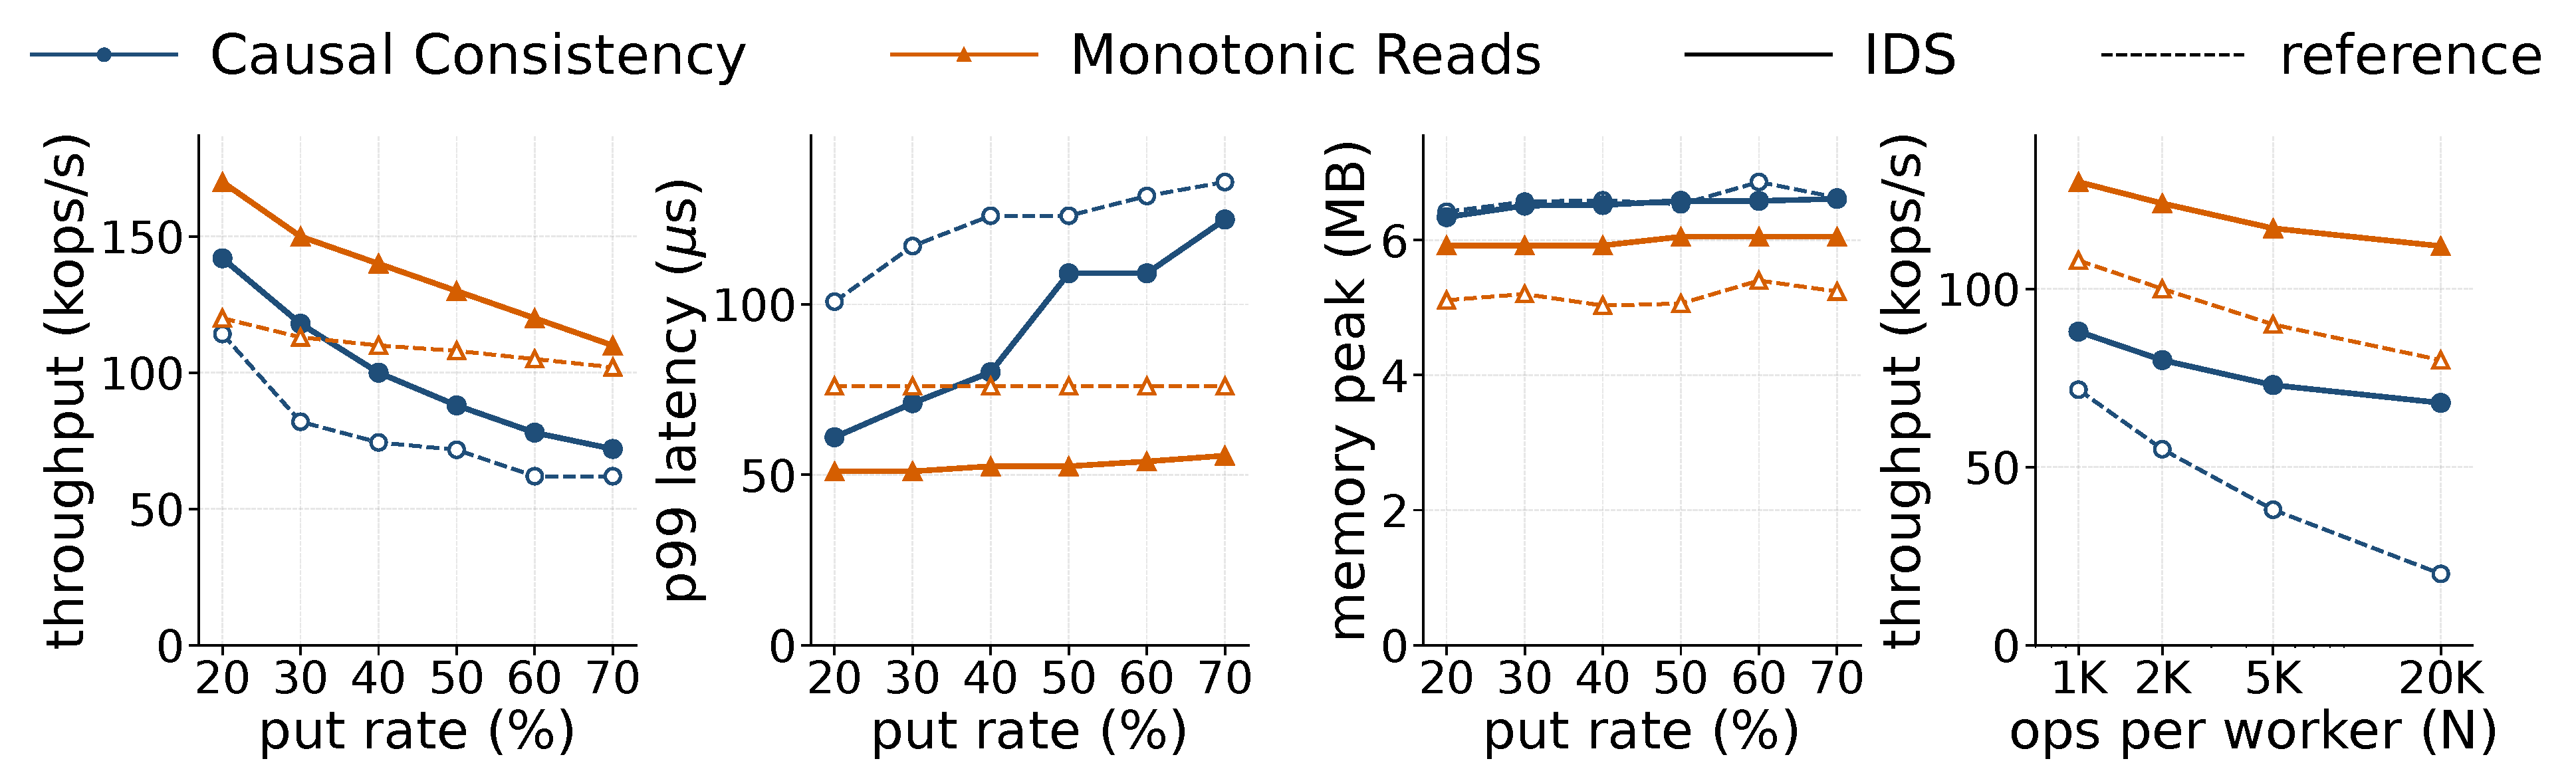
\includegraphics[width=\linewidth]{figures/eval_perf.pdf}
\caption{Throughput, p99 latency, and peak memory vs.\ put rate, and throughput vs.\ ops-per-worker $N$, for \sys{} suite CC and monotonic reads. Solid $=$ \sys{}; dashed $=$ reference (function-as-map for both). The per-spec breakdown for all seven specifications appears in
% \ion{For first and second graphs, the trends suggest that if we increase the put rate, IDS might be worse than the reference...}
% \shubham{So, Ion: as we increase puts to very high our efficiency tricks are no more useful enough and converges to the normal implementation, which btw is also a good implementation. So, maybe we can justify in that way?}
\cref{app:perf-curves}.}
\label{fig:eval-perf}
\end{figure}


\subsection{Runtime performance}
\label{sec:eval-perf}

\sys{}' synthesized implementations match or beat every prior reference: $3\times$ throughput on Chapar's vector-clock reference, $1.4\times$ on \sys{} suite CC and monotonic reads, comparable on read-your-writes (within $20\%$), and $152$k and $139$k ops/s on MW and RYW+MW where the reference times out at every put rate (\cref{app:perf-curves}). We compare on throughput, p99 latency, peak memory, and ops-per-worker scaling. Figure~\ref{fig:eval-perf} shows \sys{} suite CC and monotonic reads vs.\ the references, and 
% function-as-map
the full per-spec breakdown
% , including Chapar's vector-clock reference, 
is in \cref{app:perf-curves}. The gap follows from one mechanism: 
\sys{}' data-store representations are bounded,
% \mohsen{replaced ``bound per-op cost'' with ``are bounded''. Is that correct?} \shubham{Yes, addressed: ``are bounded'' is the cleaner framing at this abstraction level.}
% by the spec,
while the references' grow with workload size. These representations emerged from the joint code+proof loop: the proof obligation drove the agent to them (\cref{sec:eval-synthesis}). The performance feedback from the benchmark harness then steers the agent toward the fastest among multiple verifying candidates (\cref{sec:eval-ablations}).

\textbf{\sys{} suite CC. \ }
Both implementations enforce causality with one timestamp per client; the data store differs. The reference's function-from-key-to-value extracts to OCaml as a chain that grows per put (every get walks it), while \sys{} uses a balanced-tree map where a lookup costs at most the tree depth. \sys{} reaches up to $1.4\times$ peak throughput at low put rate where gets dominate, with p99 latency up to $1.7\times$ lower. 
The gap narrows at high put rate as broadcast becomes the bottleneck; tail latency tracks the same effect, rising with put rate on both implementations as broadcast queue waits grow. Peak memory is comparable at $1$k ops per worker, since the vector-clock state is bounded by client count rather than put rate; larger workloads would push it upward. On ops-per-worker scaling, the reference's throughput collapses by more than half from $1$k to $20$k ops per worker while \sys{} loses only about a quarter.


\textbf{Other \sys{} suite specifications. \ }
%
Unlike CC, these specs only need per-client guarantees, so they do not pay CC's per-write cross-client coordination cost; their tail latency stays flat across put rate (Figure~\ref{fig:eval-perf}, MR). On the other \sys{} suite specs, \sys{} ranges from comparable on read-your-writes (chain stays short) to a gap large enough that the reference times out at every put rate on the monotonic-write specs (MW, RYW+MW). 
The four with prior references (RYW, MW, MR, RYW+MW) share the closure-chain mechanism: the reference's function-from-key-to-value extracts as a chain that grows per put; \sys{} replaces it with a flat list or balanced tree, and the speedup tracks how often the chain is walked. 
% 
On the monotonic reads benchmark, a get in the reference walks every operation, so \sys{} outperforms it by $1.4\times$.

% \mohsen{The plots for the following specs is not shown in the main body. They are too detailed and should be taken to the appendix. Commented below.} \shu{Addressed: the commented detail block is dropped; per-spec plots and the RYW/MW/RYW+MW/LCC/MW-pivot detail are in \cref{app:perf-curves}.}


\subsection{Ablations and Generalization}
\label{sec:eval-ablations}

The joint step-wise discovery of code and proof is the key design decision behind \sys{}.
% The agent baselines in \cref{sec:eval-synthesis} fail because they are not step-wise.
We ablate this joint design itself ($-$J), the ISA's proposer ($-$P) and reloader ($-$R), the coordinator's audit step ($-$A), and the \coq{} feedback to the DSA ($-$VF) across the seven key-value store specs and VERINA's $189$ Lean tasks (Table~\ref{tab:eval-ablation}). We also evaluate the DSA alone and \sys{}' prover component decoupled from the rest of the system on four cross-language proof benchmarks (DafnyBench, miniCodeProps, Verus-Bench, CoqStoq), where it sets a new state-of-the-art on each.
% \accheng{mention the general prover results here} \shubham{Addressed: added preview sentence about DSA-alone cross-language results.} 

% frozen, the proof phase cannot change course.

\textbf{Architecture ablations. \ }
Without joint discovery, only RYW succeeds in a majority of runs: Chapar CC, RYW+MW, \sys{} suite CC, and LCC drop to $0$ out of $3$, and VERINA falls to $85\%$ ($-8\%$ from full \sys{}' $93\%$). This is because a fixed implementation limits the proof phase. On Chapar CC, $-$J commits to the global per-replica state closest to the spec. Full \sys{} reloads to per-key entries when the proof stalls. 
% (\cref{sec:eval-synthesis} trace). 
The audit step catches trivial solutions that pass \coq{}'s type-checker: 
on \sys{} suite CC, an agent without auditing once shipped a \texttt{put-guard} returning \texttt{false} unconditionally, with the theorem being trivially satisfied. On the other hand, cells under $-$A count only audited successful runs. 
% 
Ablations of the proposer and reloader each drop pass rate on the four hardest specs (Chapar CC, MR, \sys{} suite CC, LCC), taking VERINA to $79\%$ ($-14\%$) under $-$P and to $88\%$ ($-5\%$) under $-$R. 
% 
The \coq{} feedback to the DSA is the most consequential single component: 
replacing the structured \coq{} diagnostic (goal, hypotheses, tactic backtrace)
% \mohsen{What is structured diagnostic?} \shubham{addressed: parenthetical (goal, hypotheses, tactic backtrace) inlined.}
with only an accept/reject drops every spec to at most $1$ of $3$ successful runs and VERINA to $58\%$ ($-35\%$). 
% \shu{this reads arelaly dense, and with -J, -P, -R, which are really hard to parse... need to rephrase this to be better}
% \shu{this can be shrinked further to half a page if we are space-constrained}
% \mohsen{This paragraph is long but more readable than the previous long ones in this section.} \shu{Noted; left this paragraph as-is.}

\textbf{Performance-feedback ablation. \ }
Without performance feedback ($-$PF), the agent commits to the first implementation and proof that passes the type-checker and misses the course-corrections seen in \cref{sec:eval-perf}. 
As \cref{fig:eval-bench} shows,
full \sys{} is on average $1.42\times$ faster than $-$PF across the six specs with reference baselines (Chapar CC, RYW, MW, RYW+MW, MR, \sys{} suite CC).
% \accheng{why geomean? can we just say on average?} \shubham{Addressed: changed 'geomean' to 'on average'.}
% \mohsen{Commented the following. Why does it mean? Why do we say it?}
% The performance measurement is a search signal, not a post-hoc metric. 

\textbf{DSA as a general prover. \ }
The DSA's effectiveness is not specific to \sys{}' synthesis loop or to \coq{}: 
applied alone to public verification benchmarks across four languages, it sets a new state-of-the-art on each (Figure~\ref{fig:eval-crosslang}, Table~\ref{tab:bench-results}).
% \shu{as shown in Figure... or Table...} \shubham{Addressed: moved the (Figure, Table) citation up to this sentence.}
% It ties or beats every prior work on four public proof benchmarks across  :
It saturates miniCodeProps ($100$ of $100$) and Verus-Bench ($149$ of $150$), and beats prior SOTA by $36$ to $69\%$ on DafnyBench and CoqStoq. 
% 
% \mohsen{The following line was not clear. Replaced it with the next line.}
% The gain is the architecture, not the model: 
\sys{}' agentic architecture brings further gain:
full \sys{} adds $+10\%$ on DafnyBench, $+20\%$ on miniCodeProps, and $+51\%$ on CoqStoq over Codex under the same prompt, while a baseline-model swap (Codex $\to$ Claude under the same prompt, no \sys{} architecture) gains at most $6\%$ on any of these four benchmarks. 
% 
\sys{} also reaches state-of-the-art on all three code-and-proof benchmarks: $176/189$ on VERINA (prior SOTA $38$), $65/77$ on AlgoVeri ($2\times$ prior SOTA $31$), and a full $62/62$ on CloverBench (Table~\ref{tab:bench-results}; detail in \cref{app:benchmarks}).
% \shu{I don't like x/y this kind of writing, the number is sort of meaningless to me, maybe switch to percentage} \accheng{I would be consistent, we do say like 2 out of 7, 1 out of 3 before so maybe okay to keep. do we show the percentages in table somewhere?} \shubham{Addressed: keeping x/y per Audrey's consistency point. The paper uses x/y throughout (Q1's "2 of 7", §5.2's "3-of-3"/"2-of-3", and tables/bench-results.tex shows "176 / 189" too), so switching just these three prose lines to percentages would diverge from the tables. The "prior SOTA 38" anchor next to 176/189 makes the gap obvious without needing a percentage; "62/62" reads punchier as full saturation than "100\%".}


\begin{figure}[t]
\centering
% \begin{minipage}[b]{0.27\linewidth}
\begin{minipage}[b]{0.3\linewidth}
\centering
\providecolor{rowhl}{HTML}{EFF3F8}
\centering
% \tiny
\scriptsize
\setlength{\tabcolsep}{1.1pt}
\renewcommand{\arraystretch}{1.00}

\begin{tabular}{@{}l cccccc@{}}
\toprule
         & full & $-$J & $-$P & $-$R & $-$A & $-$VF \\
\midrule
\rowcolor{rowhl}
Chapar CC& 3/3 & 0/3 & 0/3 & 0/3 & 1/3 & 0/3 \\
RYW      & 3/3 & 2/3 & 2/3 & 3/3 & 3/3 & 1/3 \\
MW       & 3/3 & 1/3 & 2/3 & 2/3 & 2/3 & 0/3 \\
RYW+MW   & 3/3 & 0/3 & 1/3 & 2/3 & 1/3 & 0/3 \\
MR       & 3/3 & 1/3 & 0/3 & 1/3 & 0/3 & 0/3 \\
\sys{} suite CC& 2/3 & 0/3 & 0/3 & 0/3 & 0/3 & 0/3 \\
LCC      & 3/3 & 0/3 & 0/3 & 0/3 & 0/3 & 0/3 \\
\midrule
\rowcolor{rowhl}
VERINA   & 176 & 160 & 150 & 167 & 176 & 110 \\
\bottomrule
\end{tabular}
\captionof{table}{Component ablations: \# successes from $3$ runs ($189$ tasks for VERINA).}
\label{tab:eval-ablation}

\end{minipage}\hfill
% \begin{minipage}[b]{0.345\linewidth}
\begin{minipage}[b]{0.32\linewidth}
\centering
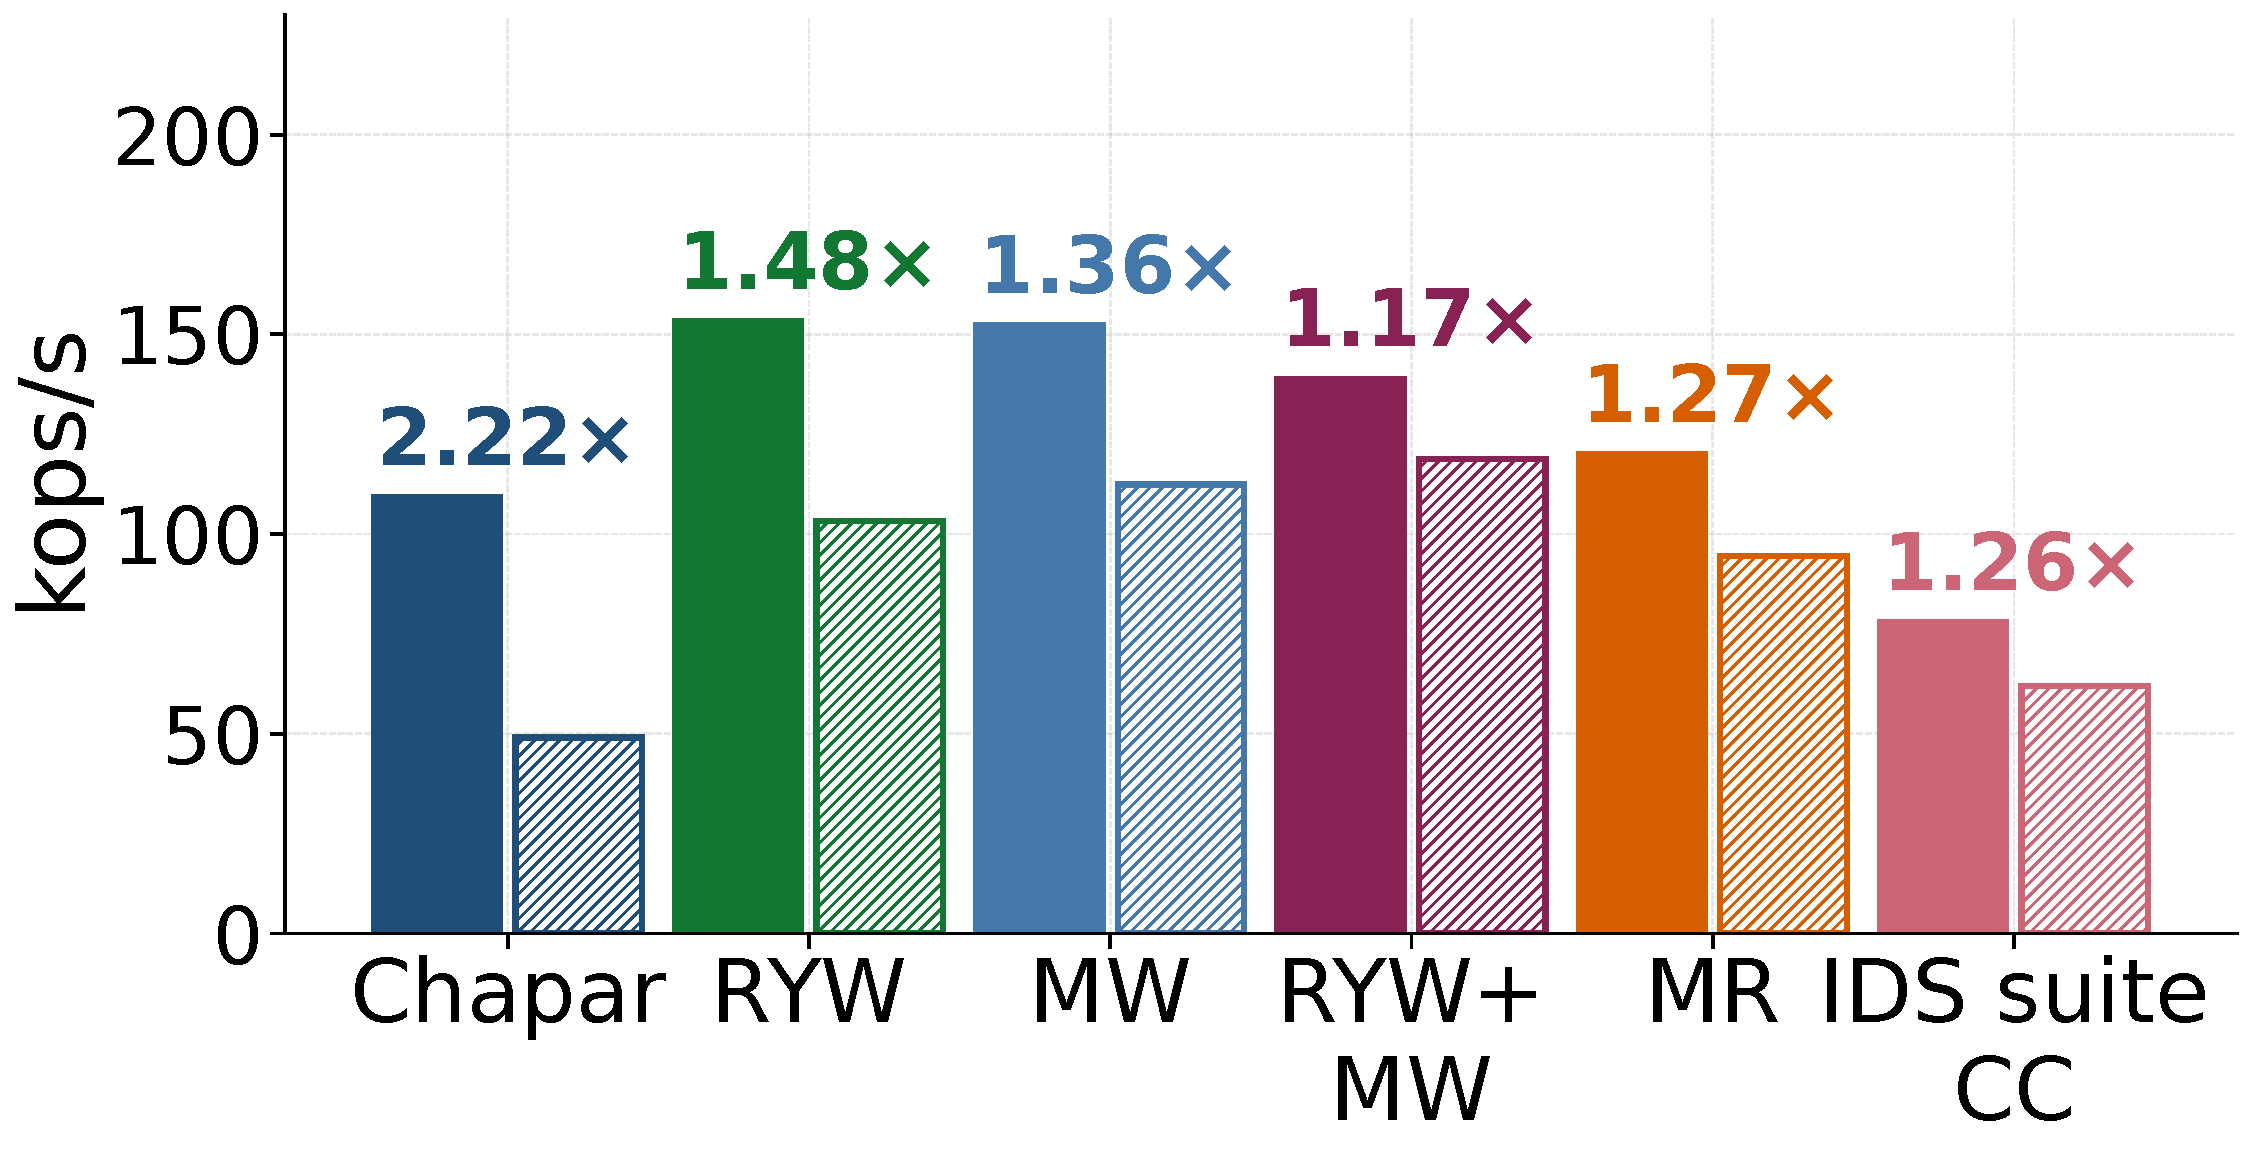
\includegraphics[width=\linewidth]{figures/eval_bench.pdf} \\[1.3em]
\captionof{figure}{Performance-feedback ablation at $\textit{put}=60\%$: \sys{} (solid) vs.\ no-feedback (hatched).}
\label{fig:eval-bench}
\end{minipage}\hfill
% \begin{minipage}[b]{0.345\linewidth}
\begin{minipage}[b]{0.32\linewidth}
\centering
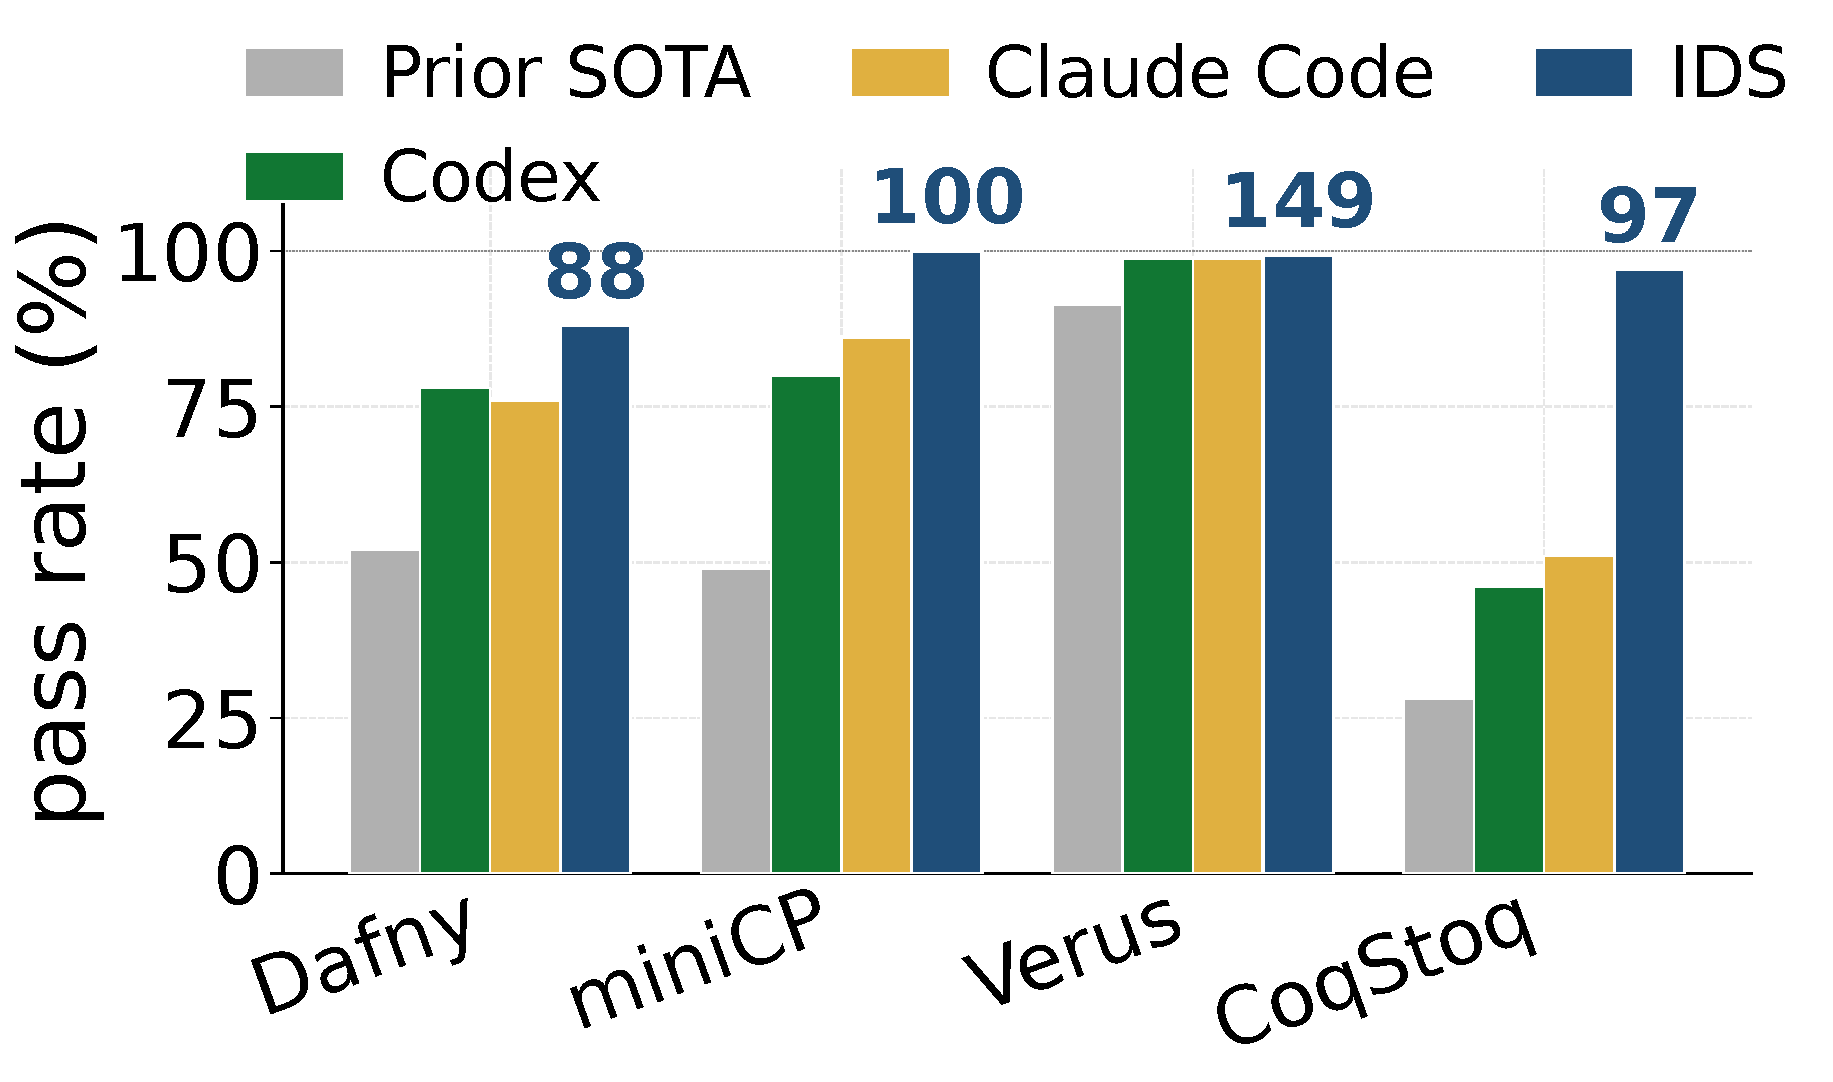
\includegraphics[width=\linewidth]{figures/eval_crosslang.pdf} %\\[0.3em]
\captionof{figure}{Cross-language success rate (\%) on 4 verification benchmarks;
labels are \# of successes.}
\label{fig:eval-crosslang}
\end{minipage}
\end{figure}




